\section{CSCH Hyperbolic Cosecant Function}

\subsection{Usage}

Computes the hyperbolic cosecant of the argument.
The syntax for its use is
\begin{verbatim}
   y = csch(x)
\end{verbatim}
\subsection{Function Internals}

The \verb|csch| function is computed from the formula
\[
   \mathrm{csch}(x) = \frac{1}{\sinh(x)}
\]
\subsection{Examples}

Here is a simple plot of the hyperbolic cosecant function
\begin{verbatim}
--> x1 = -pi+.01:.01:-.01;
--> x2 = .01:.01:pi-.01;
--> plot(x1,csch(x1),x2,csch(x2)); grid('on');
\end{verbatim}


\centerline{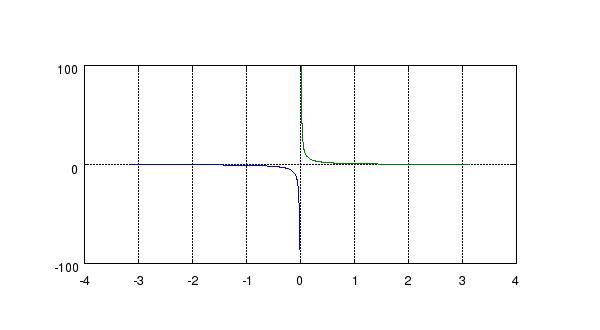
\includegraphics[width=8cm]{cschplot}}

